\documentclass{report}
\usepackage{graphicx}
\usepackage{booktabs}
\usepackage{xcolor}
\usepackage{array}
\usepackage{geometry}
\usepackage{longtable}
\usepackage{float}
\usepackage{titlesec}
\usepackage{hyperref}
\usepackage{amsmath}
\usepackage{amssymb}
\usepackage{listings}
\newcommand{\sectionbreak}{\clearpage}
 
\geometry{a4paper, margin=1in}
 
\lstset{
  basicstyle=\ttfamily\small,
  breaklines=true,
  frame=single,
}
 
\title{CROWNS Technical doc}
\author{Real Ant Engineer}
\date{May 2026}
 
\begin{document}
\maketitle

\newpage
This document gives an overview of the CROWNS mod to the Engineer Colony team, especially Artists and Developers. The goal is to explain the main simulation systems, the technical direction of the project, and the general architecture used by the mod.
\newpage

\tableofcontents

\section{Presentation, Goals, and Direction}

Crowns is a mod that aims to solve several issues found in classical nuclear power mods such as Big Reactors or Extreme Reactors. Most existing mods simplify reactor physics too much and use fixed multiblock structures with unrealistic behaviors.

The objective of CROWNS is to maintain a balance between scientific realism, gameplay readability, and acceptable computational performance.

The mod focuses on simulation depth without requiring players to have advanced scientific knowledge. Internal systems are designed to be modular so they can evolve independently over time.

The architecture separates the simulation into several large systems:
\begin{enumerate}
    \item Heat propagation.
    \item Fluid simulation.
    \item Neutron transport.
    \item Nuclear reactions and isotope transformations.
    \item Thermal Cycle
\end{enumerate}

Some subsystem, the one that are voxel based, exchanges data through shared simulation maps and chunk-based updates in order to keep acceptable performance.

\chapter{Physics and Simulation Processes}

\section{Heat propagation}

The heat system is one of the central components of the mod. Almost every machine interacts with temperature in some way. Heat affects reactor efficiency, coolant behavior and safety systems.

The simulation is volumetric. Every block stores thermal data and exchanges energy with neighboring blocks during simulation ticks.

\subsection{Differential Equation systems}

The global heat simulation can be represented as a large differential equation system.

For each block $i$, the temperature evolves as:
\[
\frac{dT_i}{dt} = \sum_j k_{ij}(T_j - T_i) + S_i
\]
where $k_{ij}$ is the heat exchange coefficient between block $i$ and its neighbor $j$, and $S_i$ is a local source term.

Assembling all $N$ blocks into a single system yields the matrix form:
\[
\frac{d\vec{T}}{dt} = A\vec{T} + \vec{S}
\]
where:
\begin{itemize}
    \item $\vec{T} \in \mathbb{R}^N$ is the temperature vector, one entry per block.
    \item $A \in \mathbb{R}^{N \times N}$ is the transfer matrix. Its off-diagonal entries $A_{ij} = k_{ij}$ encode
          heat exchange with neighbors, and its diagonal entries $A_{ii} = -\sum_{j \neq i} k_{ij} - \lambda_i$
          ensure energy conservation plus background loss.
    \item $\vec{S} \in \mathbb{R}^N$ aggregates heat sources, boundary conditions, and the background loss offset
          $\lambda_i T_{\text{env}}$.
\end{itemize}

Because each block only exchanges heat with its immediate neighbors (at most 6 in a 3D grid),
$A$ is highly sparse: each row contains at most 7 non-zero entries regardless of the total
system size. This sparsity is exploited by storing $A$ in a compressed format (CSR or similar),
reducing both memory usage and the cost of each matrix-vector product from $O(N^2)$ to $O(N)$.

\subsubsection*{Implicit discretisation}

Integrating the system explicitly (forward Euler) imposes a strict stability condition:
\[
\Delta t \leq \frac{1}{2\alpha} \frac{(\Delta x)^2}{d}
\]
where $d$ is the spatial dimension. Fine grids or highly conductive materials force very
small time steps, which is impractical for a real-time simulation.

An implicit (backward Euler) discretisation avoids this constraint. Evaluating the right-hand
side at time $t^{n+1}$ gives:
\[
\frac{\vec{T}^{n+1} - \vec{T}^{n}}{\Delta t} = A\vec{T}^{n+1} + \vec{S}
\]
Rearranging:
\[
\underbrace{(I - \Delta t\, A)}_{M} \vec{T}^{n+1} = \vec{T}^{n} + \Delta t\,\vec{S}
\]
This is a linear system $M\vec{T}^{n+1} = \vec{b}$ that must be solved at every simulation
tick. $M$ inherits the sparsity structure of $A$, so iterative solvers such as
\textbf{Conjugate Gradient} (if $M$ is symmetric positive definite) or \textbf{GMRES} are
well suited. Because the grid topology changes rarely, $M$ can be factored or preconditioned
once and reused across many ticks, keeping the per-tick cost manageable.

The simulation uses iterative numerical methods instead of analytical solutions because
the system changes continuously during gameplay.
The matrix representation also allows parallel updates and stability analysis.

\subsection{Diffusion}

Heat diffusion models heat transfer through conduction: energy moves from hotter regions to
cooler ones through direct contact, with no bulk movement of matter. It applies to solids,
stagnant fluids, and any block that does not participate in convective flow.

The governing equation is the classical diffusion equation augmented with a background loss term:
\[
\frac{\partial T}{\partial t} = \alpha \nabla^2 T - \lambda(T - T_{\text{env}})
\]
where:
\begin{itemize}
    \item $\alpha$ is the thermal diffusivity of the material, controlling how quickly heat spreads.
    \item $\lambda$ is the background loss coefficient, representing slow dissipation to the environment.
    \item $T_{\text{env}}$ is the ambient temperature.
\end{itemize}

Discretising the Laplacian $\nabla^2 T$ on the block grid with a standard second-order
finite difference stencil gives, for block $i$:
\[
(\nabla^2 T)_i \approx \frac{1}{(\Delta x)^2} \sum_{j \in \mathcal{N}(i)} (T_j - T_i)
\]
where $\mathcal{N}(i)$ is the set of face-adjacent neighbors of block $i$.
Substituting into the per-block evolution equation directly produces the entries of the
matrix $A$ described in the previous section, and the background loss $\lambda$ contributes
to both the diagonal of $A$ and the source vector $\vec{S}$ via the offset $\lambda T_{\text{env}}$.

\subsubsection*{Interface conductivity — harmonic mean}

When two blocks of different materials share a face, a single effective conductivity
$k_{\text{eff}}$ must represent the interface. Using the arithmetic mean would overestimate
heat transfer across a poorly conducting boundary. The simulation instead uses the
\textbf{harmonic mean} of the two conductivities $\kappa_i$ and $\kappa_j$:
\[
k_{\text{eff}} = \frac{2\,\kappa_i\,\kappa_j}{\kappa_i + \kappa_j}
\]
This is the exact result for two resistances in series and ensures that a single
insulating block cannot be bypassed by a highly conductive neighbor. If either
conductivity is zero the interface coefficient is set to zero, completely blocking
heat transfer across that face.

\subsubsection*{Matrix assembly — stamping}

The system matrix $M$ is assembled by iterating over every active block and
\textbf{stamping} its contribution into the global row. For each face-adjacent neighbor $j$
of block $i$, the off-diagonal coefficient is:
\[
A_{ij} = (1 - \rho)\,\gamma\, k_{\text{eff}}
\]
where $\rho$ is a numerical resistance factor and $\gamma$ is a geometry-dependent
scaling constant. The diagonal accumulates the negative sum of all outgoing coefficients
plus the background loss contribution:
\[
A_{ii} = -\sum_{j \in \mathcal{N}(i)} A_{ij} - \lambda
\]

Neighbors that lie \emph{outside} the active matrix domain (fixed-temperature boundary
blocks) are not stamped into $A$. Instead their known temperature $T_j^{\text{bc}}$ is
moved to the right-hand side:
\[
b_i \mathrel{+}= A_{ij}\, T_j^{\text{bc}}
\]
This keeps $M$ square and confined to the unknown degrees of freedom, while boundary
conditions enter cleanly through $\vec{b}$.

\subsubsection*{Material parameters}

Different materials expose three parameters that feed directly into these coefficients:
\begin{enumerate}
    \item \textbf{Thermal conductivity} $\kappa$, used to compute $k_{\text{eff}}$ at every shared face.
    \item \textbf{Background loss} $\lambda$, added to the diagonal to prevent isolated
          regions from retaining heat indefinitely and to improve matrix conditioning.
    \item \textbf{Default temperature}, used to initialise $\vec{T}$ and as the boundary
          value $T_j^{\text{bc}}$ for fixed blocks.
\end{enumerate}
This allows realistic thermal contrasts between materials such as graphite (high conductivity),
steel, concrete, and insulating blocks, purely through their parameter definitions.

\subsection{Convection}

Convection transfers heat through the bulk motion of a fluid. Unlike diffusion, it
is inherently directional: energy is carried along the local velocity field, making
it far more efficient at redistributing heat over large distances. Modelling it
accurately requires coupling the temperature field to a fluid dynamics solver.

\subsubsection*{Governing equations}

The full incompressible Navier-Stokes equations for a Newtonian fluid are:
\[
\nabla \cdot \vec{v} = 0
\]
\[
\rho \left( \frac{\partial \vec{v}}{\partial t} + (\vec{v} \cdot \nabla)\vec{v} \right)
= -\nabla p + \mu \nabla^2 \vec{v} + \vec{f}
\]
coupled to the advection-diffusion equation for temperature:
\[
\frac{\partial T}{\partial t} + \vec{v} \cdot \nabla T = D \nabla^2 T
\]
where $\vec{v}$ is the velocity field, $p$ the pressure, $\mu$ the dynamic viscosity,
$\vec{f}$ body forces (e.g.\ buoyancy), and $D$ the thermal diffusion coefficient.
Solving these equations directly (DNS) is computationally prohibitive at any useful
grid resolution. The simulation therefore adopts a \textbf{URANS} (Unsteady
Reynolds-Averaged Navier-Stokes) approximation everywhere convection occurs.

\subsubsection*{URANS approximation}

URANS decomposes every flow quantity into a time-averaged part and a fluctuating part:
\[
\vec{v} = \overline{\vec{v}} + \vec{v}', \qquad T = \overline{T} + T'
\]
Averaging the Navier-Stokes equations over a short time window eliminates the fast
turbulent fluctuations and yields equations for the mean fields only:
\[
\rho \left( \frac{\partial \overline{\vec{v}}}{\partial t}
+ (\overline{\vec{v}} \cdot \nabla)\overline{\vec{v}} \right)
= -\nabla \overline{p} + \nabla \cdot \left[(\mu + \mu_t)\nabla \overline{\vec{v}}\right] + \vec{f}
\]
\[
\frac{\partial \overline{T}}{\partial t} + \overline{\vec{v}} \cdot \nabla \overline{T}
= \nabla \cdot \left[\left(D + \frac{\nu_t}{\Pr_t}\right) \nabla \overline{T}\right]
\]
where $\mu_t$ is the turbulent eddy viscosity and $\Pr_t$ is the turbulent Prandtl number.
The effect of unresolved turbulence is absorbed into effective transport coefficients,
keeping the solved fields smooth and the system tractable at gameplay resolution.

\subsubsection*{Velocity field computation}

At each simulation tick the velocity field is solved from scratch. Fluid motion is
entirely driven by sources: blocks such as fans or pumps that inject momentum directly
into the domain. In the absence of any source the fluid is at rest.

Given the source field $\vec{f}$, the velocity field is obtained by solving the
steady-state momentum equation at each tick:
\[
\rho\,(\overline{\vec{v}} \cdot \nabla)\overline{\vec{v}}
= -\nabla \overline{p} + (\mu + \mu_t)\nabla^2 \overline{\vec{v}} + \vec{f}
\]
Pressure and density gradients then redistribute the momentum injected by sources
across the fluid domain: the pressure field $\overline{p}$ adjusts to enforce
incompressibility, and density variations due to temperature (buoyancy) tilt the
effective pressure gradient, causing hotter, lighter fluid to rise and cooler fluid
to sink. These are consequences of the momentum equation rather than independent
driving terms.

Solid boundaries are enforced by Boolean obstruction maps along each axis, which
zero out normal velocity components at blocked faces and confine the flow to the
available fluid geometry.

\subsubsection*{Coupling to the diffusion solver}

Once the velocity field is known, convective heat transport is folded into the
diffusion framework described in the previous section. The advective flux across the
face between blocks $i$ and $j$ adds an upwind term to the effective conductivity
seen by the stamping procedure:
\[
k_{\text{eff}}^{\text{conv}} = k_{\text{eff}}^{\text{cond}} + \rho\, c_p\, |\overline{v}_\perp|\, \Delta x
\]
where $\overline{v}_\perp$ is the velocity component normal to the shared face and
$c_p$ is the specific heat capacity. This term is stamped into $A$ alongside the
conductive coefficient, so both mechanisms are resolved implicitly in the same
linear system each tick.

Because the convective term breaks the symmetry of $A$, the system matrix $M$ is no
longer symmetric positive definite when convection is active. A Krylov solver such as
\textbf{GMRES} is used in place of Conjugate Gradient for fluid regions, while purely
diffusive solid regions continue to use the cheaper symmetric solver.

The simulation maintains the following data maps per fluid region:
\begin{enumerate}
    \item Fluid temperature $\overline{T}$.
    \item Density $\rho$.
    \item Viscosity $\mu$ (combined molecular and turbulent).
    \item Pressure $\overline{p}$.
    \item Velocity components $\overline{v}_x$, $\overline{v}_y$, $\overline{v}_z$.
    \item Boolean obstruction maps along $x$, $y$, and $z$.
\end{enumerate}

\section{Phase change and fluid circuits}

The thermodynamic state of a fluid is fully described by two independent properties.
The simulation uses enthalpy $H$ and pressure $P$ as its primary state variables,
as they are naturally conserved in the transport processes modelled by the fluid circuit.

\subsection{Thermodynamic tables}

Rather than solving equations of state at runtime, the simulation precomputes four
two-dimensional lookup tables for water:
\begin{enumerate}
    \item $(P, H) \rightarrow T$ — temperature.
    \item $(P, H) \rightarrow S$ — specific entropy.
    \item $(P, H) \rightarrow X$ — vapour quality (liquid--vapour fraction).
    \item $(P, S) \rightarrow H$ — enthalpy from pressure and entropy.
\end{enumerate}
These four tables are sufficient to resolve any thermodynamic transformation encountered
in the circuit. Each table is stored as a regular 2D grid and evaluated at runtime by
bilinear interpolation between the four nearest nodes.

Queries that fall outside the table bounds can produce artefacts due to extrapolation
with a linear scheme. A planned improvement replaces the current tables with
\textbf{spline-based isobaric and isoenthalpic contour tables}, which better capture
the curvature of the thermodynamic surface near saturation and remain well-behaved when
the operating point drifts outside the precomputed domain.

\subsection{Fluid transport}

Mass and enthalpy are transported through the circuit using the pipe and pump
infrastructure provided by the \textit{Create} mod. Three types of thermodynamic
process are modelled:

\begin{enumerate}
    \item \textbf{Isobaric heating — heat exchanger.} Pressure is held constant while
          enthalpy increases or decreases through the exchanger walls. The state moves
          horizontally in the $(P, H)$ plane; the new temperature and vapour quality are
          read directly from the $(P,H) \rightarrow T$ and $(P,H) \rightarrow X$ tables.

    \item \textbf{Isentropic compression or expansion — compressor and turbine.}
          Entropy is conserved across the machine. The outlet enthalpy is obtained by
          first reading $S$ from the $(P,H) \rightarrow S$ table at inlet conditions,
          then evaluating the $(P,S) \rightarrow H$ table at the outlet pressure with
          the same entropy value.

    \item \textbf{Transport — pipes and pumps.} Fluid is moved between components with
          no heat exchange and no work input beyond what the pump provides to raise
          pressure. The pump work $W = \Delta P / \rho$ is added to the enthalpy of
          the fluid parcel.
\end{enumerate}

Together these three primitives allow the construction of arbitrary Rankine or
Brayton cycles directly in the game world, with thermodynamic consistency maintained
throughout by the table lookups.

\section{Neutron Transport}

The neutron transport system is responsible for reactor criticality and nuclear reactions.
Classical nuclear mods often use simplified adjacency rules where reactor behavior depends
only on neighboring blocks. In these systems, neutrons are not physically simulated and
interactions are reduced to local bonuses or penalties.

CROWNS instead models neutron propagation using ray tracing. Neutrons travel through reactor
geometry, interact probabilistically with materials, and can be absorbed, moderated, reflected,
or escape the system entirely.

\subsection{Cross-sections}

The probability of a neutron triggering a fission event in a material is quantified by
its \textbf{microscopic fission cross-section} $\sigma_f$ (measured in barns,
$1\,\text{b} = 10^{-28}\,\text{m}^2$). The macroscopic fission cross-section for a
material of atomic number density $N$ is:
\[
\Sigma_f = N \sigma_f
\]
and governs the mean free path $\ell = 1/\Sigma_f$ between fission events.

The simulation distinguishes two neutron energy groups: \textbf{thermal} and \textbf{fast}.
Each fissile material stores a pair of values $(\sigma_{\text{thermal}},\, \sigma_{\text{fast}})$
sourced from tabulated nuclear data. During ray tracing, the appropriate value is selected
based on whether the neutron has been moderated or not.

Fission cross-sections are also temperature-dependent. This dependence is modelled through
an inverse law in fuel temperature $T$:
\[
\sigma_f(T) \propto \frac{1}{T}
\]
so that hotter fuel presents a smaller effective fission cross-section to incoming neutrons,
reducing the fission rate and damping the chain reaction. This constitutes a natural
negative temperature coefficient: a power surge heats the fuel, which lowers $\sigma_f$,
which reduces the fission rate and stabilises the reactor.

The current implementation has several limitations. Scattering and absorption are not
modelled as distinct interaction channels: all neutron-material interactions are resolved
as fission events, which neglects parasitic capture and moderation within the fuel itself.
The two-group energy discretisation is also coarse; a finer multi-group treatment would
require storing cross-section values as a \texttt{float[]} indexed by group rather than
as a fixed pair, with a shared global \texttt{float[]} specifying the energy boundary of
each group. This structure would be both more memory-efficient and more cache-friendly
during ray traversal, and would allow the number of energy groups to be extended without
changes to the material data format.

\subsection{Ray tracing}

Neutron propagation is simulated by casting rays through the voxel geometry. Each ray
represents a neutron history and is traced step by step through the material grid.

At each step the survival probability after travelling a distance $s$ through a uniform
material is:
\[
P(\text{survival}) = e^{-\Sigma_t\, s}
\]
where $\Sigma_t = \Sigma_a + \Sigma_s$ is the total macroscopic cross-section. A random
free path $\ell$ is sampled from the exponential distribution:
\[
\ell = -\frac{\ln \xi}{\Sigma_t}, \qquad \xi \sim \mathcal{U}(0,1)
\]
When the neutron reaches its interaction site, a second random draw selects the
interaction type with probabilities proportional to the partial cross-sections. The
four possible outcomes are:
\begin{enumerate}
    \item \textbf{Fission} — the neutron is absorbed and the fission routine is triggered,
          depositing energy and emitting prompt neutrons into the next generation.
    \item \textbf{Absorption} — the neutron is captured without fission, transmuting the
          target nucleus.
    \item \textbf{Scattering} — the neutron continues in a new direction with reduced energy,
          as determined by the moderator's scattering kernel.
    \item \textbf{Escape} — the ray exits the tracked geometry and the neutron is lost.
\end{enumerate}

This approach naturally handles complex reactor geometries and arbitrary fuel arrangements
without any adjacency heuristics, giving the player full freedom in reactor design.

\section{Nuclear Equations}

Nuclear reactions are implemented as transformation maps:
\[
\text{Isotope} \xrightarrow{\text{reaction}} \sum_i \text{Product}_i
\]
Each reaction entry defines:
\begin{enumerate}
    \item Input isotopes and their stoichiometric coefficients.
    \item Output isotopes and their yields.
    \item Released energy $Q$.
    \item Prompt and delayed neutron production $\nu$.
\end{enumerate}

\subsection{Burnup and isotope evolution}

Isotope evolution is driven by two independent processes, each governed by its own equation.

\subsubsection*{Neutron-induced fission}

When a fissile nucleus captures a neutron, it undergoes fission. The consumed quantity
of isotope $k$ during a simulation step $\Delta t$ is:
\[
\Delta N_k = \xi_k\, N_k^n, \qquad \xi_k = 1 - e^{-\Sigma_f \phi\, \Delta t}
\]
where $\phi$ is the local neutron flux and $\Sigma_f$ is the macroscopic fission
cross-section of the material. The advancement value $\xi_k \in [0,1]$ represents
the reacted fraction of the isotope during the step. Output isotopes and energy $Q$
are then accumulated proportionally to $\Delta N_k$ according to the reaction table.
A representative example:
\[
^{235}\text{U} + n \;\rightarrow\; ^{141}\text{Ba} + ^{92}\text{Kr} + 3n + Q
\]

\subsubsection*{Natural decay}

Unstable isotopes decay spontaneously with a characteristic half-life $t_{1/2}$,
independently of any neutron flux. The surviving fraction after a step $\Delta t$ is
given by the radioactive decay law:
\[
\Delta N_k = N_k^n \left(1 - e^{-\lambda_k \Delta t}\right), \qquad
\lambda_k = \frac{\ln 2}{t_{1/2}}
\]
where $\lambda_k$ is the decay constant of isotope $k$. The daughter nuclei and
any emitted energy are accumulated in the same way as fission products.

Both processes run independently each simulation step and can act on the same isotope
simultaneously: a fission product may be both produced by fission and consumed by its
own decay within the same tick.

\subsection{Registry and extensibility}

Internally, isotopes are stored in a global registry and reactions are loaded from
dynamic reaction tables at startup. Adding a new nuclear chain — a novel fuel cycle,
a breeding reaction, or an activation product — requires only a new data entry and no
changes to the simulation core.

This architecture supports:
\begin{itemize}
    \item \textbf{Fuel burnup} — fissile inventory depletes as the reactor operates.
    \item \textbf{Breeding} — fertile isotopes such as $^{238}$U or $^{232}$Th convert
          to fissile material under neutron irradiation.
    \item \textbf{Waste management} — fission products and actinides accumulate,
          affecting reactivity and requiring reprocessing or disposal.
\end{itemize}


\chapter{Gameplay Considerations}

\section{Minerals, Metals and Ingredients}

The mod introduces a small set of materials chosen to cover the essential steps of a
nuclear fuel cycle without attempting to reproduce the full periodic table.

Uranium is the primary fissile resource. It is collected as an ore found underground
and as a byproduct of washing quartz. Raw uranium is first converted into uranium
hexafluoride by mixing it with glowstone dust, then processed a second time to separate
depleted uranium from enriched uranium. This enrichment step is currently handled in a
generic mixer but would benefit from a dedicated centrifuge block, both for realism and
to give the separation process a more distinct identity in the production chain.

Plutonium is produced inside the reactor through neutron capture in depleted uranium.
It serves as fuel for RTGs and as the fissile core of nuclear devices, with a potential
secondary use as blaze burner fuel under consideration.

Titanium provides structural and shielding materials used in instruments and radiation
barriers. Boron is consumed by control rods. Cobalt-64 acts as a portable neutron
source, useful for starting or probing a reactor.

Because the number of distinct in-game items is finite, most fission products cannot
be given their own physical representation in the player's inventory. Any isotope that
does not correspond to a named item in the registry is aggregated into radioactive waste,
a catch-all material that still carries heat and radiation properties and must be managed
accordingly. The underlying simulation tracks the full reaction chain regardless; the
simplification is purely at the item level.

\section{Turbine}

The current turbine block has two practical problems. Its mandatory casing is visually
restrictive and limits creative freedom in plant layouts, while being functionally inert:
it neither seals the flow path nor creates a pressure differential between stages. A
first improvement would allow the casing requirement to be disabled, or alternatively
to detect a player-built enclosure — a sealed volume defined by surrounding blocks —
and treat that as the aerodynamic boundary, rewarding intentional construction without
enforcing a specific aesthetic.

Stage progression is another area for improvement. With a fixed maximum of 16 stages,
each stage index can be stored directly in the block state and given a dedicated model,
providing clear visual feedback on how far the working fluid has expanded through the
machine. A stator block would complement this by allowing the player to alternate rotor
and stator rows, closer to real turbine design.

\begin{figure}[H]
    \centering
    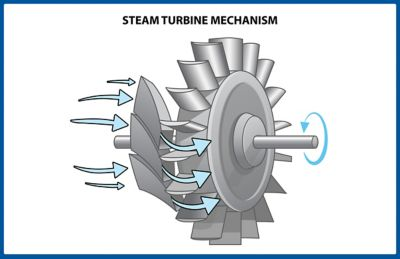
\includegraphics[width=0.5\linewidth]{images/turbine/stator_rotor.png}
    \caption{Stator and rotor arrangement.}
    \label{fig:turbine-stator-rotor}
\end{figure}

\begin{figure}[H]
    \centering
    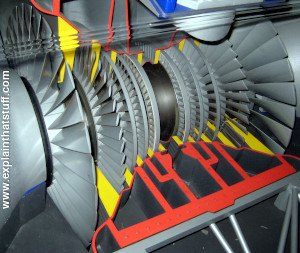
\includegraphics[width=0.5\linewidth]{images/turbine/stages.png}
    \caption{General idea of stage progression.}
    \label{fig:turbine-stages}
\end{figure}

\subsection{Reactor Control Rods}

Currently reactor rods are made with gold blocks with either mechanical piston or pulleys.
Its problematic because it's hard to detect moving contraption inside the raycasting (or a diffusion algorithme if we use an approximation in the future), it would be nicer for the player and cleaner for the devs to use dedicated control rods blocks, it would require making an abstraction for rods. here is how it would work :
a rod can go through blocks that are "hollow", (either air or a block that can reasive a control rod) based on the surfaced block we can scale the moderation, absorption or anything that the rod is meant to impact. The block will render the control rod with a block entity allowing for smooth transition bwn position.
That way we can graphite tipped graphite rods.

An other proposed idea would be the sliding door fuel assembly, it's something that kinda exist in aerospace but with rotating drums. It has to been said that it's less realistic and the proposing was controversial.

\begin{figure}[H]
    \centering
    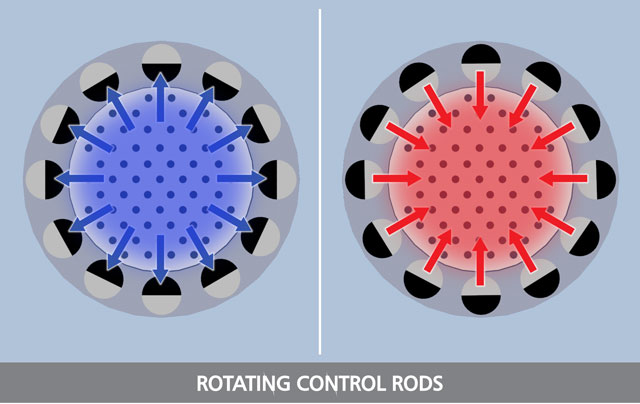
\includegraphics[width=0.5\linewidth]{images//reactor/rotating_rods.png}
    \caption{Rotating "control rods"}
    \label{fig:placeholder}
\end{figure}

\begin{figure}[H]
    \centering
    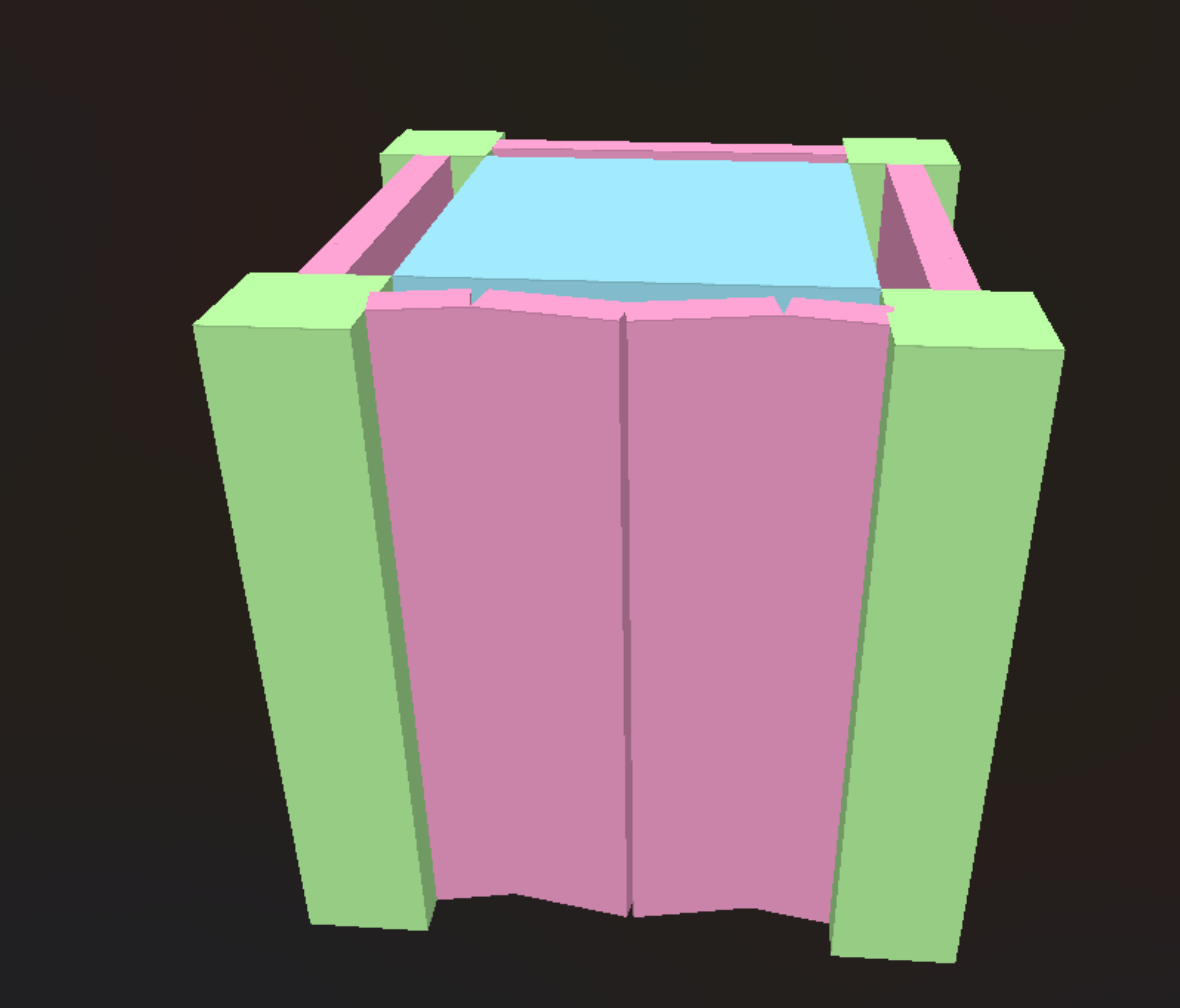
\includegraphics[width=0.5\linewidth]{images//reactor/sliding_door.png}
    \caption{Sliding door proposed version}
    \label{fig:placeholder}
\end{figure}

\subsection{Reactor Damage}

The current failure model transitions the reactor directly from a fully operational state
to an explosion or meltdown with no intermediate warning, giving the player no opportunity
to intervene. A progressive damage system would make accidents feel more grounded and
actionable. Damage would accumulate over time under abnormal operating conditions —
analogous to the durability model used by anvils — and manifest through observable
symptoms before any catastrophic event: gas leaks, unusual sounds, rising readings on
the monitoring panel. This graduated escalation gives the player a window to perform an
emergency shutdown, repair damaged components... Accumulated damage state would also be
exposed through the reactor monitor, allowing attentive players to catch degradation
early.

\section{QoL and Explanations}

\subsection{Reactor Design}

Designing a working reactor layout requires understanding neutron geometry, moderation,
and criticality — none of which are easy to reason about inside the game. A dedicated
design tool, either an external web application in the spirit of the Big Reactors
simulator (\href{https://br.sidoh.org}{br.sidoh.org}) or a simulator integrated directly
into the mod's interface, would allow players to iterate on layouts before committing
materials. An integrated solution has the advantage of access to the exact cross-section
tables and geometry rules used by the simulation, giving accurate predictions rather than
approximations.

\subsection{Physics Primer}

The frequency of basic questions about cycle layout — such as where to place the
compressor relative to the turbine — indicates that the thermodynamic principles
underlying the mod are not self-evident. Ponder scenes explaining how a Rankine or
Brayton cycle works, what entropy and enthalpy represent in practical terms, and why
stage order matters would significantly lower the barrier to entry without simplifying
the underlying simulation.

\section{Monitoring}

\subsection{Reactor Monitoring}

A reactor information panel should allow the player to select any fuel rod and read its
current isotopic composition, burnup state, and local neutron flux. Derived quantities
such as the doubling time, the prompt-to-delayed neutron ratio, and the effective
multiplication factor $k_{\text{eff}}$ would give experienced players a meaningful
stability margin to work with. Control rod insertion depth should also be readable from
the same interface. On the instrumentation side, a neutron detector block would allow
in-world flux mapping without opening any GUI.

\subsection{Cycle Monitoring}

Cycle efficiency is difficult to assess without a thermodynamic state diagram.
Displaying the operating point of each major component — boiler, turbine, condenser,
pump — on a Mollier ($H$--$S$) diagram in real time would let players immediately see
where irreversibilities occur and how far the cycle deviates from the ideal isentropic
case.

\subsection{Temperature and Flow Visualisation}

The current temperature overlay displays values as text labels, which becomes unreadable
at any useful scale. Replacing it with a colour map — a continuous thermal palette
applied directly to block faces or as a screen overlay — would make hot spots and thermal
gradients immediately legible. Fluid velocity deserves a similar treatment: a vector
field overlay is straightforward to implement and conveys direction, while streamlines
would give a cleaner picture of large-scale circulation patterns at the cost of
additional computation.

\section{Harmful Effects}

\subsection{Temperature}

Extreme temperatures reuse Minecraft's existing burning and freezing mechanics together
with their standard countermeasures, keeping the system familiar to players and avoiding
redundant implementation work.

\subsection{Radiation}

Radiation exposure causes acute radiation syndrome. The current implementation on the
\texttt{1.20.1-dev} branch applies a constant nausea effect and periodic health loss
scaled to the received dose. The CROWNS addon addresses a similar problem and should be
reviewed before further development to avoid duplicating solutions and to assess whether
integration or interoperability is feasible.

\end{document}